\chapter{Results}
\label{chap:results}
The results presented here are after training the networks for $\sim$400 epochs (~5.5 hours) on approximately 300,000 2D poses with a batch size of 2560 on an Nvidia Titan X. The input poses are flipped with a probability of 0.5. The model takes 16 joints as the output where the root is added at the origin for validation. The proposed architecture consists 1024 hidden units per linear layer and 51 latent dimensions. Both the \ac{vae} and the discriminator are trained using Adam optimizer with default hyperparameters and with a learning rate of 2e-4. The gradient norms of the discriminator is clipped to 1 when training the discriminator. While training the generator the gradient norms are clipped to 2 for all the models while the gradient values are clipped to 1000.

One of the challenging parts is finding the optimal weights for each of the terms in the triplet loss. The loss coefficients $\lambda_{recon}$, $\lambda_{\acs{kld}}$, $\lambda_{disc.}$ are set to 1, 0.001, 0.001 respectively. The higher weight is motivated by 2 reasons. $\lambda_{recon}$ refers to the constrained optimization and irrespective of how realistic it is, projection loss is desired to be consistently low to get better \ac{mpjpe}. That leads to the other reason that the quantitative results are given higher importance.
%TODO add loss standardization values to kld

The values of $\lambda{\acs{kld}}$ and $\lambda{disc.}$ can be tuned according to the task at hand based on how well the poses are to be clustered or how important it is to reject poses that are not realistic. The $\beta$ value for the \ac{vae} is cycled from 0 to $\lambda_{\acs{kld}}$ every 40 epochs. While keeping it constant at $\lambda_{\acs{kld}}$ for 10 epochs with a 10 epoch warmup at the beginning of the training.

\section{Quantitative Results}

The results obtained by the networks with the above configuration in addition to the choices mentioned in \ref{chap:experiments} are summarized in Table \ref{table:result_zv}. The summaries of the models are provided in appendix \ref{chap:summaries} to help reproduction.

\begin{table}[htb!]
    \centering
    \begin{tabularx}{\linewidth}{XXX}%{llcc}
        \toprule
        Supervision  & Algorithm                               & Error (mm) \\
        \midrule \midrule
        Full         & Martinez \etal \cite{MartinezHRL17}     & 37.1       \\
                     & Chen \etal \cite{multiplehypo} (SH, MH) & 42.6       \\
        \midrule
        Weak         & Wandt \etal \cite{repnet}               & 38.2       \\
                     & Drover \etal \cite{can3dpose}           & 38.2       \\
                     & Chen \etal \cite{weaklymultiple} (SH)   & 48.7       \\
                     & Chen \etal \cite{weaklymultiple} (BH)   & 31.6       \\
        \midrule
        Unsupervised & Ching \etal \cite{amazon1}              & 58         \\
                     & Ching \etal \cite{amazon1} (AD) (TD)    & 51         \\
                     & \textbf{Ours}                           & 52.4       \\
                     & \textbf{Ours} (BH)                        & 50         \\
        \bottomrule
    \end{tabularx}
    \caption{}
    \label{table:result_zv}
    \vspace{-3ex}
\end{table}

\textbf{SH} refers to the results using 2D Stacked Hourglass detections as input. These detections are noisy and directly affects the predictions of the model. And \textbf{DA} refers to using Domain Adaptation network to include additional datasets and \textbf{TD} denotes the use of temporal data. It is important to note that the proposed unsupervised method and the one presented in \cite{amazon1} are the only methods that do not predict the scale of the 3D pose due to the processing technique.

\begin{table}[h]
    \centering
    \begin{tabularx}{\textwidth}{llllllll}
        R\_Hip & R\_Knee & R\_Ankle    & L\_Hip   & L\_Knee  & L\_Ankle    & Torso    & Neck \\
        \hline
        58.01  & 61.42   & 81.97       & 52.45    & 60.13    & 92.82       & 44.78    & 25.43 \\
        &&&&&&&\\
        Nose   & Head    & L\_Shoulder & L\_Elbow & L\_Wrist & R\_Shoulder & R\_Elbow & R\_Wrist\\
        \hline
        33.39  & 46.29   & 30.48       & 55.72    & 80.84    & 33.53       & 59.23    & 80.05\\
    \end{tabularx}
    \caption{Average per joint position error (in mm) for each joint under Protocol $\#2$ using 2D ground truth.}
    \label{table:pjpe}
\end{table}

The best hypothesis, \textbf{BH} has improved the results by ~2.7 mm which is considerable in comparison to the equivalent gain in \cite{amazon1} using domain adaptation network with more data and temporal information. Since there is no technique to pick the best hypothesis without having access to the ground truth, the results referred to, are the ones obtained using \textbf{ZV} unless specified otherwise. The average \ac{mpjpe} using ZV, 52.74mm, is equivalent to the settings of \cite{amazon1} without additional data or temporal information, 58 mm. This is a significant improvement considering that the network from \cite{amazon1} only predicts the depth, cannot handle missing points, gives a single hypothesis, and uses a self-symmetry technique that takes twice as many training iterations for equivalent network complexity. Fig \ref{fig:mpjpe_trends} illustrates the distribution of the \ac{mpjpe} errors for each action.

\begin{figure}[h]
    \centering
    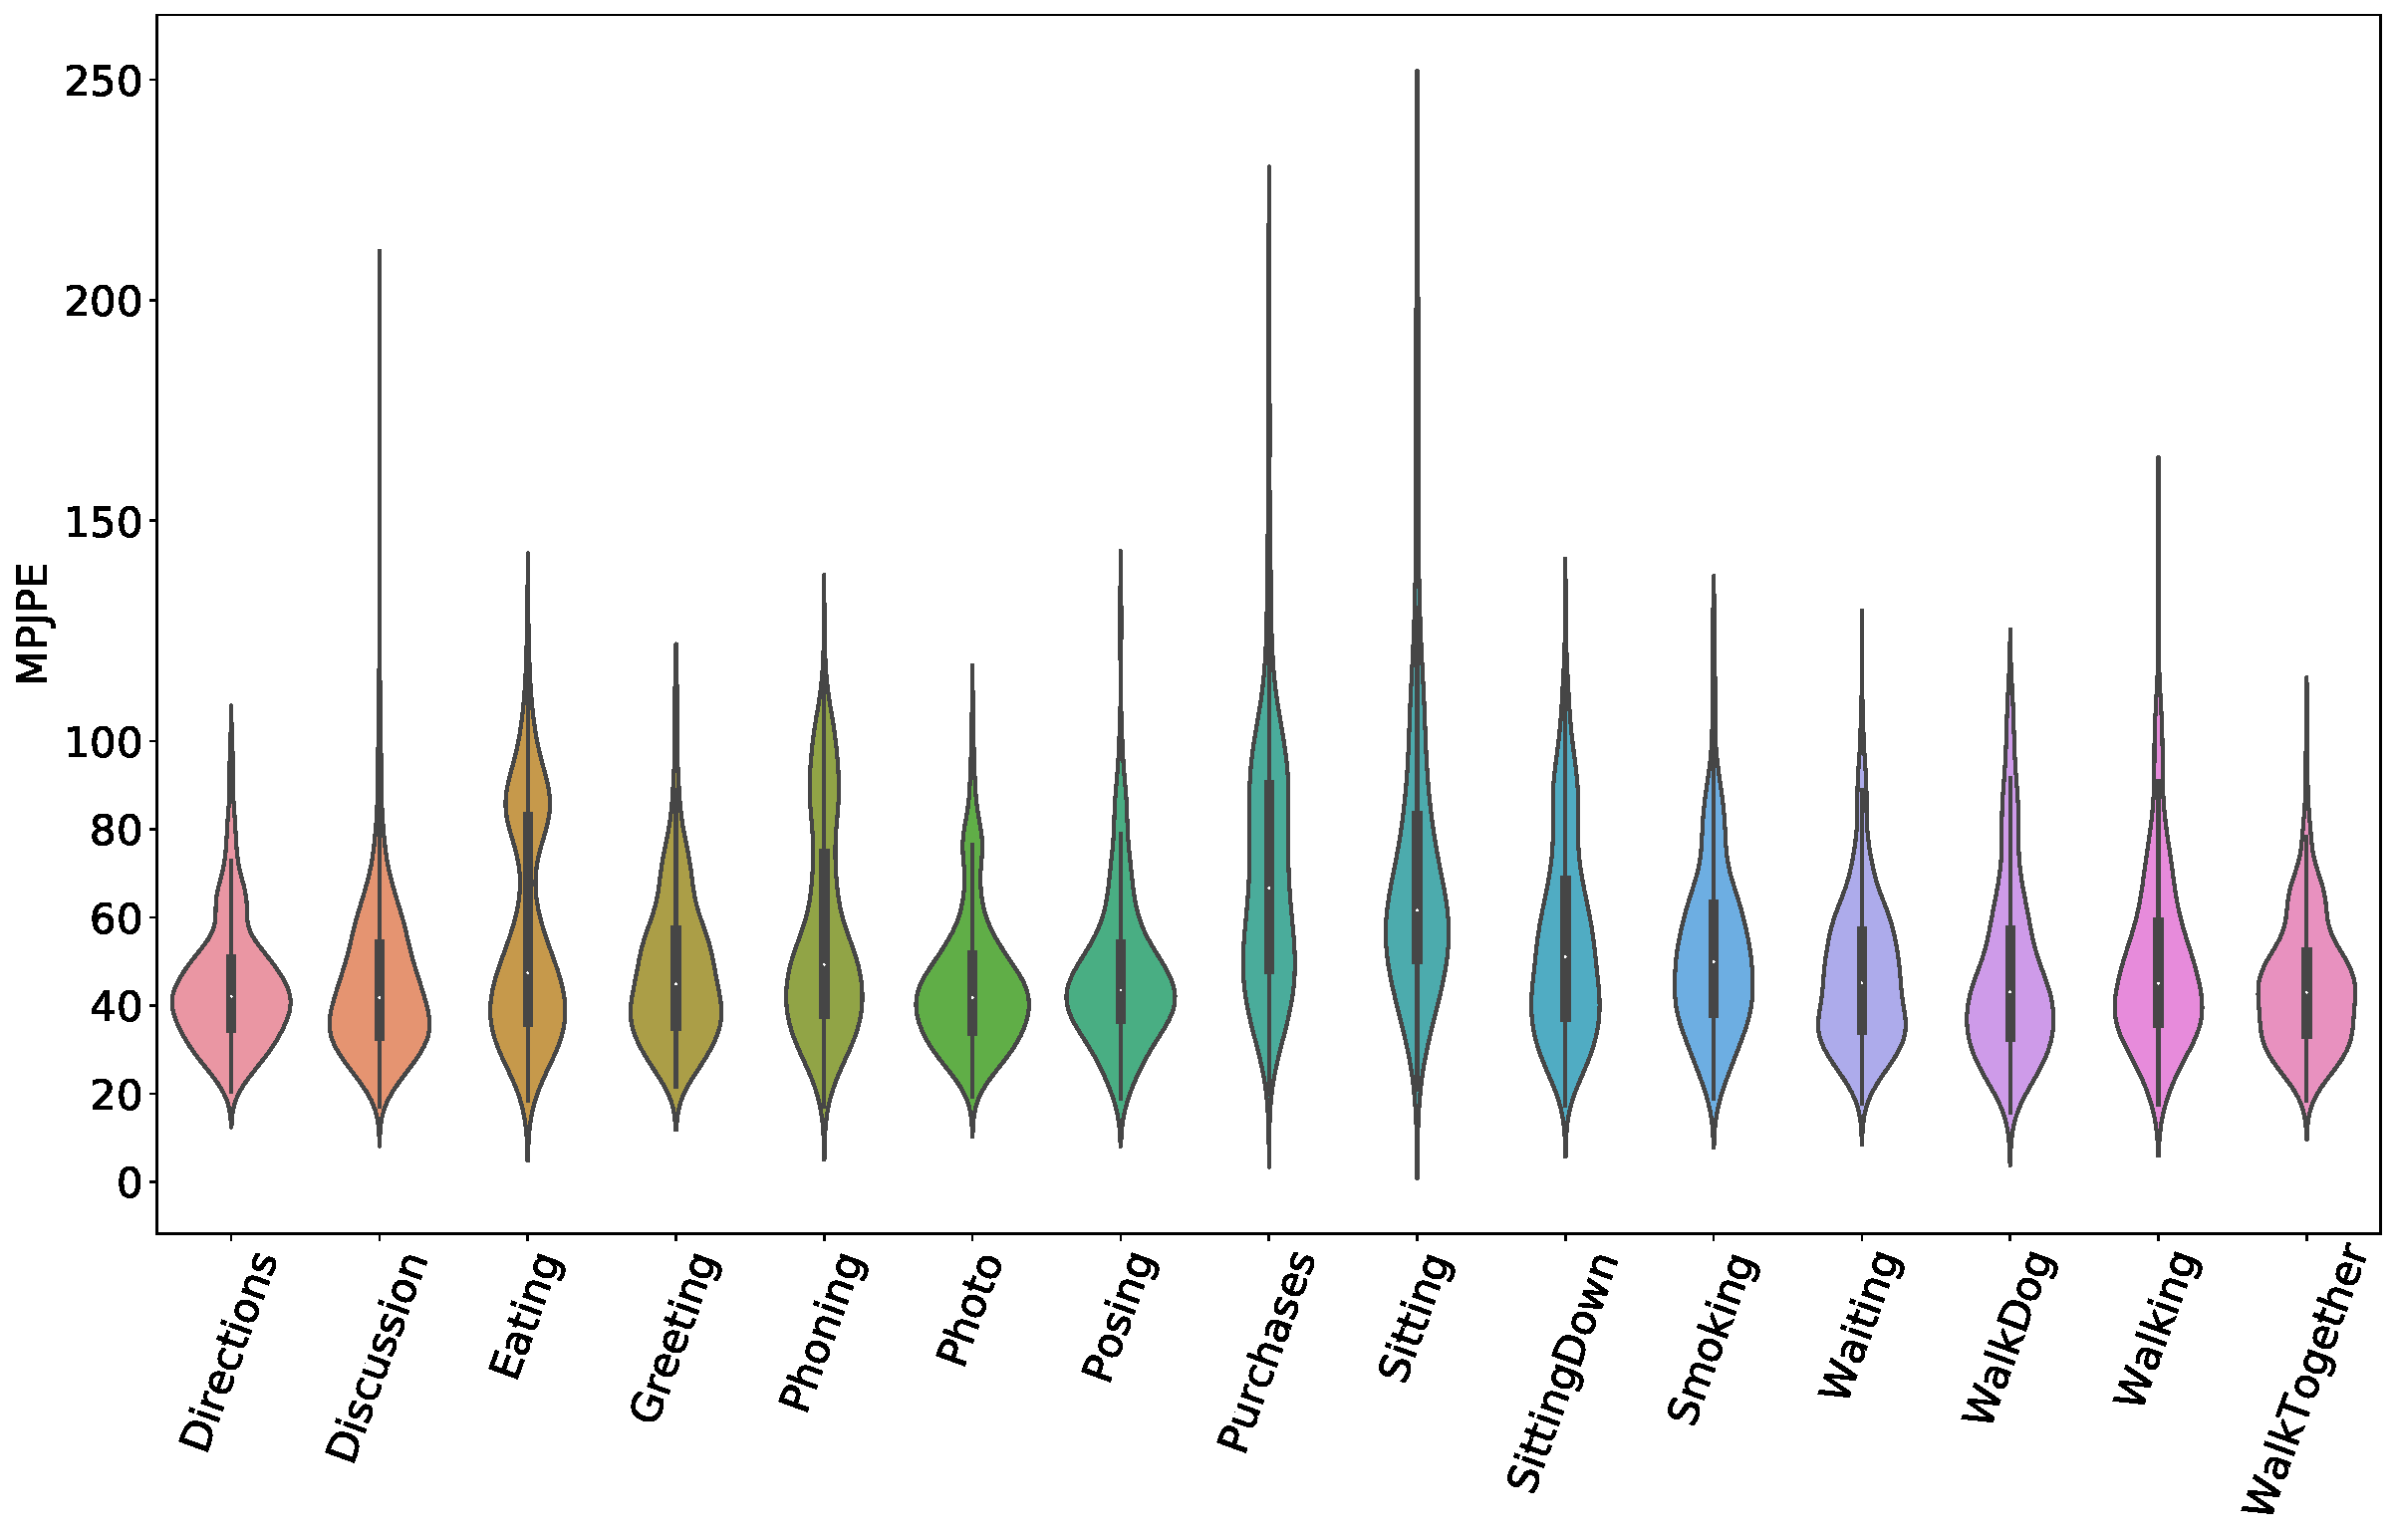
\includegraphics[width=\textwidth]{figures/results/violin_pjpe.pdf}
    \caption{Visualization of the MPJPE error distribution under Protocol $\#2$ for each action.}
    \label{fig:mpjpe_trends}
\end{figure}

The \ac{mpjpe} error per joint increases as we move from inner to outer joints. This can be observed in Table \ref{table:pjpe} which shows the average per joint position error. The error in the limb joints is due to the larger variation in their location through out the data compared to joints like the neck or the nose. Moreover, these joints are often occluded by the person's body especially when doing actions such as sitting. The 2D projections a pose from sitting posture is clustered to a smaller region from certain \acp{pov}. This makes it challenging to estimate the scale and depth of each joint and leads to outliers as visualized in the violin plots.

Since the data consists an equal mix of data from different \acp{pov}, the predictions from the \ac{pov}, where the limbs are in the \ac{fov} are more informative than the other \acp{pov}. When the limbs are not in the \ac{fov}, the model learns to guess their location based on other features such as articulation or posture of the body. The effect of \ac{pov} is the possible cause of the bimodal error distribution in actions such as purchases, eating, phoning. Since the actions are hands specific, they are restricted to a particular region making the pose more predictable from one \ac{pov} and less from another. These challenges are inherent to the task of pose lifting and in many cases is challenging even for a human eye.

\section{Qualitative Results}

\newcommand{\inp}[1]{figures/zv_mean/#1_inp.png}
\newcommand{\pred}[1]{figures/zv_mean/#1_pred.png}
\newcommand{\gt}[1]{figures/zv_mean/#1_gt.png}

\newif\ifreal 
% \realtrue

\begin{figure}[h!]
    \centering
    \ifreal
    \begin{subfigure}[b]{0.45\textwidth}
        \includegraphics[width=0.3\textwidth]{\inp{3493}}
        \includegraphics[width=0.3\textwidth]{\pred{3493}}
        \includegraphics[width=0.3\textwidth]{\gt{3493}}
        % \caption*{Directions - 44.44mm}
    \end{subfigure}
    \begin{subfigure}[b]{0.45\textwidth}
        \includegraphics[width=0.3\textwidth]{\inp{6422}}
        \includegraphics[width=0.3\textwidth]{\pred{6422}}
        \includegraphics[width=0.3\textwidth]{\gt{6422}}
        % \caption*{Discussion - 44.49mm}
    \end{subfigure}
    
    
    \begin{subfigure}[b]{0.45\textwidth}
        \includegraphics[width=0.3\textwidth]{\inp{14027}}
        \includegraphics[width=0.3\textwidth]{\pred{14027}}
        \includegraphics[width=0.3\textwidth]{\gt{14027}}
        % \caption*{Eating - 56.63mm}
    \end{subfigure}
    \begin{subfigure}[b]{0.45\textwidth}
        \includegraphics[width=0.3\textwidth]{\inp{74176}}
        \includegraphics[width=0.3\textwidth]{\pred{74176}}
        \includegraphics[width=0.3\textwidth]{\gt{74176}}
        % \caption*{Greeting - 49.15mm}
    \end{subfigure}
    
    
    \begin{subfigure}[b]{0.45\textwidth}
        \includegraphics[width=0.3\textwidth]{\inp{21621}}
        \includegraphics[width=0.3\textwidth]{\pred{21621}}
        \includegraphics[width=0.3\textwidth]{\gt{21621}}
        % \caption*{Phoning - 56.59mm}
    \end{subfigure}
    \begin{subfigure}[b]{0.45\textwidth}
        \includegraphics[width=0.3\textwidth]{\inp{26692}}
        \includegraphics[width=0.3\textwidth]{\pred{26692}}
        \includegraphics[width=0.3\textwidth]{\gt{26692}}
        % \caption*{Photo - 44.22mm}
    \end{subfigure}
    
    
    \begin{subfigure}[b]{0.45\textwidth}
        \includegraphics[width=0.3\textwidth]{\inp{30089}}
        \includegraphics[width=0.3\textwidth]{\pred{30089}}
        \includegraphics[width=0.3\textwidth]{\gt{30089}}
        % \caption*{Posing - 46.50mm}
    \end{subfigure}
    \begin{subfigure}[b]{0.45\textwidth}
        \includegraphics[width=0.3\textwidth]{\inp{33987}}
        \includegraphics[width=0.3\textwidth]{\pred{33987}}
        \includegraphics[width=0.3\textwidth]{\gt{33987}}
        % \caption*{Purchases - 71.16mm}
    \end{subfigure}
    
    
    \begin{subfigure}[b]{0.45\textwidth}
        \includegraphics[width=0.3\textwidth]{\inp{39416}}
        \includegraphics[width=0.3\textwidth]{\pred{39416}}
        \includegraphics[width=0.3\textwidth]{\gt{39416}}
        % \caption*{Sitting - 72.55mm}
    \end{subfigure}
    \begin{subfigure}[b]{0.45\textwidth}
        \includegraphics[width=0.3\textwidth]{\inp{94650}}
        \includegraphics[width=0.3\textwidth]{\pred{94650}}
        \includegraphics[width=0.3\textwidth]{\gt{94650}}
        % \caption*{SittingDown - 55.01mm}
    \end{subfigure}
    
    
    \begin{subfigure}[b]{0.45\textwidth}
        \includegraphics[width=0.3\textwidth]{\inp{96348}}
        \includegraphics[width=0.3\textwidth]{\pred{96348}}
        \includegraphics[width=0.3\textwidth]{\gt{96348}}
        % \caption*{Smoking - 51.98mm}
    \end{subfigure}
    \begin{subfigure}[b]{0.45\textwidth}
        \includegraphics[width=0.3\textwidth]{\inp{54005}}
        \includegraphics[width=0.3\textwidth]{\pred{54005}}
        \includegraphics[width=0.3\textwidth]{\gt{54005}}
        % \caption*{Waiting - 47.79mm}
    \end{subfigure}
    
    
    \begin{subfigure}[b]{0.45\textwidth}
        \includegraphics[width=0.3\textwidth]{\inp{55495}}
        \includegraphics[width=0.3\textwidth]{\pred{55495}}
        \includegraphics[width=0.3\textwidth]{\gt{55495}}
        % \caption*{WalkDog - 46.86mm}
    \end{subfigure}
    \begin{subfigure}[b]{0.45\textwidth}
        \includegraphics[width=0.3\textwidth]{\inp{106863}}
        \includegraphics[width=0.3\textwidth]{\pred{106863}}
        \includegraphics[width=0.3\textwidth]{\gt{106863}}
        % \caption*{Walking - 48.73mm}
    \end{subfigure}
    
    \begin{subfigure}[b]{0.45\textwidth}
        \includegraphics[width=0.3\textwidth]{\inp{109473}}
        \includegraphics[width=0.3\textwidth]{\pred{109473}}
        \includegraphics[width=0.3\textwidth]{\gt{109473}}
        % \caption*{WalkTogether - 44.00mm}
    \end{subfigure}
    \else
        \includegraphics[width=\textwidth]{example-grid-100x100pt}
    \fi
    \caption{Visualization of (left to right) the input 2D poses with RGB background for reference, the predicted 3D pose after Procrustes alignment (in blue) and the ground truth 3D pose (in pink). The aligned predictions are the ones closest to the \textbf{mean} MPJPE error of each action.}
    \label{fig:zv_mean}
\end{figure}




















% \newcommand{\inp}[1]{figures/zv_fail/fails_#1_inp.png}
\newcommand{\pred}[1]{figures/zv_fail/fails_#1_pred.png}
\newcommand{\gt}[1]{figures/zv_fail/fails_#1_gt.png}


\begin{figure}[h]
    \centering
    \begin{subfigure}[b]{0.45\textwidth}
        \includegraphics[width=0.3\textwidth]{\inp{2878}}
        \includegraphics[width=0.3\textwidth]{\pred{2878}}
        \includegraphics[width=0.3\textwidth]{\gt{2878}}
        % \caption*{Directions - 44.44mm}
    \end{subfigure}
    \begin{subfigure}[b]{0.45\textwidth}
        \includegraphics[width=0.3\textwidth]{\inp{6130}}
        \includegraphics[width=0.3\textwidth]{\pred{6130}}
        \includegraphics[width=0.3\textwidth]{\gt{6130}}
        % \caption*{Discussion - 44.49mm}
    \end{subfigure}



    \begin{subfigure}[b]{0.45\textwidth}
        \includegraphics[width=0.3\textwidth]{\inp{73047}}
        \includegraphics[width=0.3\textwidth]{\pred{73047}}
        \includegraphics[width=0.3\textwidth]{\gt{73047}}
        % \caption*{Eating - 56.63mm}
    \end{subfigure}
    \begin{subfigure}[b]{0.45\textwidth}
        \includegraphics[width=0.3\textwidth]{\inp{18120}}
        \includegraphics[width=0.3\textwidth]{\pred{18120}}
        \includegraphics[width=0.3\textwidth]{\gt{18120}}
        % \caption*{Greeting - 49.15mm}
    \end{subfigure}



    \begin{subfigure}[b]{0.45\textwidth}
        \includegraphics[width=0.3\textwidth]{\inp{24801}}
        \includegraphics[width=0.3\textwidth]{\pred{24801}}
        \includegraphics[width=0.3\textwidth]{\gt{24801}}
        % \caption*{Phoning - 56.59mm}
    \end{subfigure}
    \begin{subfigure}[b]{0.45\textwidth}
        \includegraphics[width=0.3\textwidth]{\inp{26722}}
        \includegraphics[width=0.3\textwidth]{\pred{26722}}
        \includegraphics[width=0.3\textwidth]{\gt{26722}}
        % \caption*{Photo - 44.22mm}
    \end{subfigure}



    \begin{subfigure}[b]{0.45\textwidth}
        \includegraphics[width=0.3\textwidth]{\inp{31669}}
        \includegraphics[width=0.3\textwidth]{\pred{31669}}
        \includegraphics[width=0.3\textwidth]{\gt{31669}}
        % \caption*{Posing - 46.50mm}
    \end{subfigure}
    % \begin{subfigure}[b]{0.45\textwidth}
    %     \includegraphics[width=0.3\textwidth]{\inp{34930}}
    %     \includegraphics[width=0.3\textwidth]{\pred{34930}}
    %     \includegraphics[width=0.3\textwidth]{\gt{34930}}
    % \caption*{Purchases - 71.16mm}
    % \end{subfigure}
    % \begin{subfigure}[b]{0.45\textwidth}
    %     \includegraphics[width=0.3\textwidth]{\inp{90950}}
    %     \includegraphics[width=0.3\textwidth]{\pred{90950}}
    %     \includegraphics[width=0.3\textwidth]{\gt{90950}}
    %     % \caption*{Sitting - 72.55mm}
    % \end{subfigure}
    \begin{subfigure}[b]{0.45\textwidth}
        \includegraphics[width=0.3\textwidth]{\inp{43450}}
        \includegraphics[width=0.3\textwidth]{\pred{43450}}
        \includegraphics[width=0.3\textwidth]{\gt{43450}}
        % \caption*{SittingDown - 55.01mm}
    \end{subfigure}



    \begin{subfigure}[b]{0.45\textwidth}
        \includegraphics[width=0.3\textwidth]{\inp{98756}}
        \includegraphics[width=0.3\textwidth]{\pred{98756}}
        \includegraphics[width=0.3\textwidth]{\gt{98756}}
        % \caption*{Smoking - 51.98mm}
    \end{subfigure}
    \begin{subfigure}[b]{0.45\textwidth}
        \includegraphics[width=0.3\textwidth]{\inp{101351}}
        \includegraphics[width=0.3\textwidth]{\pred{101351}}
        \includegraphics[width=0.3\textwidth]{\gt{101351}}
        % \caption*{Waiting - 47.79mm}
    \end{subfigure}



    \begin{subfigure}[b]{0.45\textwidth}
        \includegraphics[width=0.3\textwidth]{\inp{105002}}
        \includegraphics[width=0.3\textwidth]{\pred{105002}}
        \includegraphics[width=0.3\textwidth]{\gt{105002}}
        % \caption*{WalkDog - 46.86mm}
    \end{subfigure}
    \begin{subfigure}[b]{0.45\textwidth}
        \includegraphics[width=0.3\textwidth]{\inp{106047}}
        \includegraphics[width=0.3\textwidth]{\pred{106047}}
        \includegraphics[width=0.3\textwidth]{\gt{106047}}
        % \caption*{Walking - 48.73mm}
    \end{subfigure}


    \begin{subfigure}[b]{0.45\textwidth}
        \includegraphics[width=0.3\textwidth]{\inp{61221}}
        \includegraphics[width=0.3\textwidth]{\pred{61221}}
        \includegraphics[width=0.3\textwidth]{\gt{61221}}
        % \caption*{WalkTogether - 44.00mm}
    \end{subfigure}

    \caption{Left to right are the input 2D poses with RGB reference, the predicted 3D pose (in blue) and the ground truth 3D pose (in pink). The aligned predictions are the ones closest to the mean MPJPE error of every action.}
    \label{table:zv_fail}
\end{figure}



















\begin{figure}[h]
    \centering
    \includegraphics[width=\textwidth]{example-grid-100x100pt}
    \caption{(a) Prediction on hard poses with hih ambiguity. (b) Poses that can be improved with changes to data processing.}
    \label{fig:bad_samples}
\end{figure}



Some of such outliers are presented in fig \ref{fig:bad_samples}, the predictions in (a) are the ones the model is unable to learn. While (b) is the evidence of the shortcoming of the current processing technique. Rectifying that would improve the evaluation metric of the model quite significantly.



\section{Latent Space}

% begin{figure}[h]
% \centering
%     \includegraphics[width=\textwidth]{figures/results/umap.pdf}
%     \caption{ UMAP Visualization of samples in latent space. The actions do not always directly related to the pose due to overlaps from one action to another. Better viewed in color and zoomed}
% \label{fig:latentspace}
% \end{figure}

% %reference c3dpo
\newcommand{\methtext}[1]{\centering\scriptsize\hspace{0.01cm}{\hspace{0.2cm}#1}\hspace{0.02cm}}
\newcommand{\inpC}[1]{figures/neighbours/#1_2d.png}


\newif\ifreal 
% \realtrue

\begin{figure}[h]
    \centering
    \ifreal
    \begin{tabular}{p{0.15\textwidth}p{0.85\textwidth}}
        \methtext{\textbf{\color[RGB]{66,154,201}Query Pose}} &
        \methtext{\textbf{\color[RGB]{66,154,201}Nearest Neighbours in Latent Space}} \\
    \end{tabular}
    \begin{subfigure}[b]{\textwidth}
        \fbox{\includegraphics[width=0.16\textwidth]{\inpC{7817}}}
        \includegraphics[width=0.16\textwidth]{\inpC{7742}}
        \includegraphics[width=0.16\textwidth]{\inpC{7123}}
        \includegraphics[width=0.16\textwidth]{\inpC{6102}}
        \includegraphics[width=0.16\textwidth]{\inpC{7752}}
        \includegraphics[width=0.16\textwidth]{\inpC{5484}}
    \end{subfigure}
    \begin{subfigure}[b]{\textwidth}
        \fbox{\includegraphics[width=0.16\textwidth]{\inpC{3418}}}
        \includegraphics[width=0.16\textwidth]{\inpC{2850}}
        \includegraphics[width=0.16\textwidth]{\inpC{6441}}
        \includegraphics[width=0.16\textwidth]{\inpC{3279}}
        \includegraphics[width=0.16\textwidth]{\inpC{7194}}
        \includegraphics[width=0.16\textwidth]{\inpC{7126}}
    \end{subfigure}
    \begin{subfigure}[b]{\textwidth}
        \fbox{\includegraphics[width=0.16\textwidth]{\inpC{7126}}}
        \includegraphics[width=0.16\textwidth]{\inpC{7264}}
        \includegraphics[width=0.16\textwidth]{\inpC{7254}}
        \includegraphics[width=0.16\textwidth]{\inpC{7386}}
        \includegraphics[width=0.16\textwidth]{\inpC{7237}}
        \includegraphics[width=0.16\textwidth]{\inpC{7108}}
    \end{subfigure}
    \begin{subfigure}[b]{\textwidth}
        \fbox{\includegraphics[width=0.16\textwidth]{\inpC{7043}}}
        \includegraphics[width=0.16\textwidth]{\inpC{3079}}
        \includegraphics[width=0.16\textwidth]{\inpC{2895}}
        \includegraphics[width=0.16\textwidth]{\inpC{3125}}
        \includegraphics[width=0.16\textwidth]{\inpC{2888}}
        \includegraphics[width=0.16\textwidth]{\inpC{2909}}
    \end{subfigure}
    \begin{subfigure}[b]{\textwidth}
        \fbox{\includegraphics[width=0.16\textwidth]{\inpC{791}}}
        \includegraphics[width=0.16\textwidth]{\inpC{5617}}
        \includegraphics[width=0.16\textwidth]{\inpC{6755}}
        \includegraphics[width=0.16\textwidth]{\inpC{826}}
        \includegraphics[width=0.16\textwidth]{\inpC{629}}
        \includegraphics[width=0.16\textwidth]{\inpC{8435}}
    \end{subfigure}
    \else
    \includegraphics[width=\textwidth]{example-grid-100x100pt}
    \fi
    \caption{The first pose in box is the query 2D pose and the following 5 2D poses are its nearest neighbors in the latent space.}
    \label{fig:neighbors}
\end{figure}


The visualization of 2D pose embedding in latent space after dimensionality reduction using \ac{umap} is shown in fig. \ref{fig:latentspace}. Each action is given a unique color. Though we small clusters of blues, browns, pinks the overall space looks very mixed up. This is expected as many of the instances in different actions overlap. For example, the action standing up and sitting down have instances while both or standing or sitting, etc.



% \section{missing joints}
